%
%----------------------------------------------------------------------------------------
%	PACKAGES AND DOCUMENT CONFIGURATIONS
%----------------------------------------------------------------------------------------
%
\documentclass[12pt]{article} %report, article, amsart, exam
\usepackage[letterpaper,margin=1in]{geometry}
\usepackage{fancyhdr,color}
\usepackage{tikz,graphicx,multicol}
\usepackage{amssymb,euscript,eufrak,nicefrac,enumitem}
\usepackage{amsfonts,amsmath,amsthm} %don't need with 'amsart' document class
\usepackage{hyperref}
\usepackage{comment}
\usepackage{scrextend} %needed for addmargin environment
\usepackage{graphicx} 
\usepackage{listings}
\usepackage{color}
\usepackage{accsupp}
\usepackage{booktabs}
\usepackage{subcaption}


\definecolor{dkblue}{rgb}{0,0,0.5}
\definecolor{comment}{rgb}{1,0,0}
\definecolor{mauve}{rgb}{.627,.126,.941}
\definecolor{purple}{rgb}{0.5, 0, 0.545098}


%
%----------------------------------------------------------------------------------------
%% Define headers & footers
%----------------------------------------------------------------------------------------

\pagestyle{fancy}
   \lhead{} 
   %\chead{Loyola University Chicago} 
   \rhead{}
   \renewcommand{\headrulewidth}{0pt}
   \addtolength{\footnotesep}{5mm}
%
%----------------------------------------------------------------------------------------
%% Some user-defined colors
%----------------------------------------------------------------
\setlength{\parskip}{1em}
\renewcommand{\baselinestretch}{1.3}
%
%----------------------------------------------------------------------------------------
%% BEGIN: topmatter
%----------------------------------------------------------------------------------------
%
\title{ COMP 488 - Machine Learning \\ Perceptron \& Adaline Algorithms} % Title
\author{
Loyola University Chicago \\
Jose Luis Rodriguez 
} % Author name
\date{\today} % Date for the report
%
%% END: topmatter
%%------------------------------
\begin{document}
\maketitle
\thispagestyle{fancy}

%---------------------------------------------------------------------------------------- 
%	SECTION 1 - PROBLEM STATEMENT
%----------------------------------------------------------------------------------------

\section{Overview}
This report highlights the steps to build two different datasets one linearly separable the other non-separable in order to apply the Perceptron machine algorithm to these two datasets to record it's performance and accuracy. Finally a similar algorithm called Adeline ( ADAptive LInear NEuron classifier ) is used on the Titanic dataset in order to predict passenger survival. This report was generated using python (Version 3.6.1) and the following packages:

\begin{itemize}
\item \textbf{Numpy:}  A the fundamental package for scientific computing with Python.
\item \textbf{Matplotlib:} A Python 2D plotting library which produces publication quality figures 
\item \textbf{Sckitlearn:} Simple and efficient tools for data mining and data analysis
\end{itemize}

\subsection{Python Code}
This report also provides a python (Version 3.6.1) code that creates the two datasets and prints out in the terminal the results of the Perceptron and Adeline algorithm. It only uses the following standard machine learning libraries -- Numpy to create and manipulate data and Sckit-learn to normalize and create a train-test split of the Titanic dataset.

%----------------------------------------------------------------------------------------
%	SECTION 2 - PERCEPTRON ALGO ON SEPARABLE DATA
%----------------------------------------------------------------------------------------

\section{Classification -- Linear Separable Data}

As part of the data preparation process a linearly separable dataset was generated by taking a sample from two normal distributions (Figure.1) with different mean ($\mu$) and standard deviation ($\sigma$).

\begin{figure}[htb]
\caption{Sample Normal Distributions}\label{fig:barplots01}
\hspace*{-1.9cm}
    \begin{subfigure}[b]{0.6\textwidth}
        %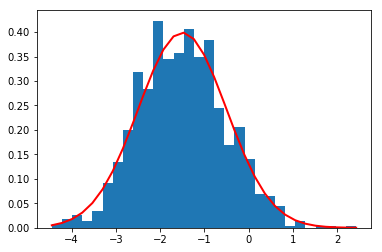
\includegraphics[width=\textwidth]{imgs/output_0.png}
        \caption{Sampla A -- Mean = -1.5, sd = 1}
        \label{fig:output_0}
    \end{subfigure}
    \begin{subfigure}[b]{0.6\textwidth}
        %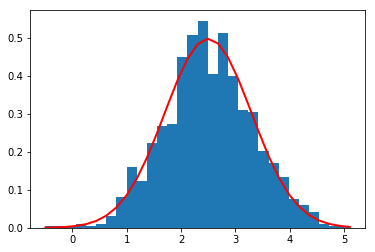
\includegraphics[width=\textwidth]{imgs/output_1.png}
        \caption{Sampla B -- Mean = 2.5 , sd = 0.8}
        \label{fig:output_1}
    \end{subfigure}
\end{figure}


In Table.1 we can see the simulated dataset that contains three columns two are features and one contains the labels to classify each observation, the shape of the data consist of 200 rows and 3 columns. By sampling from the two normal distributions above we can generate a dataset that follows a normal distribution. The class labels are $-1$ and $1$ which follows the requirements of the Perceptron algorithm that uses such labels to update its weights in order to converge. 

\begin{table}[ht]
\centering
\caption{Simulated Separable Data  - Shape (Columns, Rows): (3, 200)}
\begin{tabular}{@{}lll@{}}
\toprule
\textbf{feature\_0} & \textbf{feature\_1} & \textbf{class\_label} \\ \midrule
2.5734 & -1.0201 & 1 \\
1.7487 & -0.4891 & 1 \\
2.3314 & -0.825 & 1 \\
4.2478 & 2.2008 & -1 \\
3.2073&3.402& -1\\
2.6468&3.3961&-1\\ \bottomrule
\end{tabular}
\end{table}


When creating a dataset from scratch to test the Perceptron algorithm there are a couple of challenges that we can encounter. From intuition we can we can just plot the data and see how the different classes are distributed and if we can make an linear division between the two classes. In the case of the Perceptron algorithm there should an ideal linear division as if the gap between of the classes is too wide the algorithm would not be able to divide the data between the two classes successfully its also very important that the labels used to identify class are given by $1$ and $-1$ as these numeric labels are important during the weights update of the Perceptron algorithm.

In Figure.2a we can see the distribution of the entries in the feature-1 variable, as we can see both follow a normal distribution and because each variable was drawn from a normal distribution with different mean and standard deviation it is unlikely that the two would overlap making the dataset non separable. Now on Figure.2b we are plotting the two features part of the linearly separable dataset from the plot we can see that the two classes don't overlap each other making it possible to use the Perceptron algorithm to separate the two classes.

\begin{figure}[ht]
\caption{Linearly Separable Dataset Plots}\label{fig:linear01}
\hspace*{-1.9cm}
    \begin{subfigure}[b]{0.6\textwidth}
        %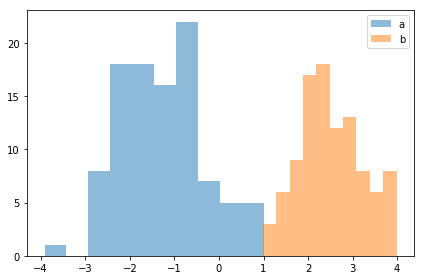
\includegraphics[width=\textwidth]{imgs/output_2.png}
        \caption{Histogram of Feature-1 by Class Label }
        \label{fig:output_2}
    \end{subfigure}
    \begin{subfigure}[b]{0.6\textwidth}
        %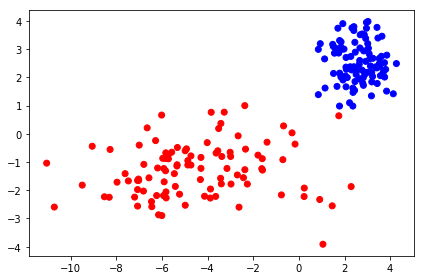
\includegraphics[width=\textwidth]{imgs/output_3.png}
        \caption{Datasets Scatter Plot by Color Class Label}
        \label{fig:output_3}
    \end{subfigure}
\end{figure}

\subsection{Perceptron Model Training on Linear Separable Data}

With the dataset ready and properly label we can use the Perceptron implementation on the book \textit{Python Machine Learning} by \textit{Sebastian Raschka} to train a model using the Perceptron algorithm to separate the data in two classes. When training the perceptron model there are some parameters that we need to input into the model in order to ensure that the algorithm converges. Table.2 shows the number of iteration (Epochs) and the errors in each iteration when training the Perceptron model on the linear separable dataset. 

\begin{table}[ht]
\centering
\caption{Perceptron Model - No. Iterations and Errors per Iterations}
\begin{tabular}{@{}lllllllllll@{}}
\toprule
\textbf{Epochs}     & 0 & 1 & 2 & 3 & 4 & 5 & 6 & 7 & 8 & 9 \\ \midrule
\textbf{No. Errors} & 1 & 3 & 2 & 1 & 0 & 0 & 0 & 0 & 0 & 0 \\ \bottomrule
\end{tabular}
\end{table}

This parameters are learning rate ($eta=0.45$) this is the rate to update the weights during each training cycle and the number of runs (Epochs) to train the model ($n\_iter = 10$). It is important to note that these parameters arent standard and there is some previous tuning in order to achieve convergence. From the plot No.updates vs. Epochs below (Figure.3) we can visualize the how the Perceptron algorithm converges after 5 iterations (Epochs).

\begin{figure}[ht]
\caption{Training the Perceptron Model}\label{fig:Perceptron01}
\centering
%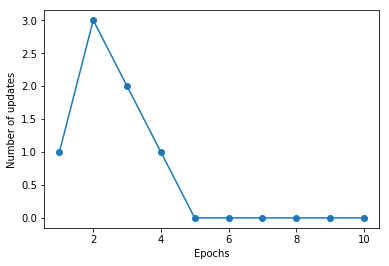
\includegraphics[width=13cm,height=12cm,keepaspectratio]{imgs/output_4.png}
\end{figure}

Finally when we can determine that the Perceptron algorithm converged after $n$ runs, meaning that the algorithm was able to successfully separate the dataset in two classes. We can plot the two features (features\_0 and features\_1) in the data against each other and draw a decision boundary line, below in Figure.4 the two features are colored coded and the decision boundary separates the two classes.

\begin{figure}[ht]
\caption{Perceptron Model Decision Boundary }\label{fig:Perceptron02}
\centering
%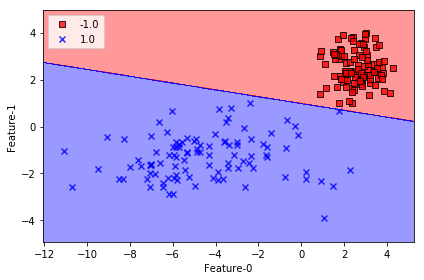
\includegraphics[width=13cm,height=12cm,keepaspectratio]{imgs/output_5.png}
\end{figure}

%----------------------------------------------------------------------------------------
%	SECTION 3 - DATA PREPARATION AND ANALYSIS
%----------------------------------------------------------------------------------------

\section{Classification -- Non-Linear Separable Data}

Following the same procedure to create linear separable data below is the non-linear simulated dataset in the same shape as the previous dataset three columns two of them are features and one contains the labels to classify each observation (200 rows and 3 columns). Similarly the two normal distributions were sampled to generate a dataset of non-linear separable data that follows a normal distribution. The class labels requirement is the same ($-1$, $1$) which updates the Perceptron weights based until the algorithm converges. 

\begin{table}[ht]
\centering
\caption{Simulated Non-Separable Data  -- Shape (Columns, Rows): (3, 200)}
\begin{tabular}{@{}lll@{}}
\toprule
\textbf{feature\_0} & \textbf{feature\_1} & \textbf{class\_label} \\ \midrule
3.0495	&	-0.4231	&	1	\\
3.7905	&	0.8824	&	1	\\
3.9684	&	-3.3438	&	1	\\
2.4916	&	2.2821	&	-1	\\
2.6468	&	3.8961	&	-1	\\
4.061	&	2.8626	&	-1	\\ \bottomrule
\end{tabular}
\end{table}

In the case of non-linear separable data we can see that the distribution of the entries in the feature-1 variable, also follow a normal distribution but in this case there were some modification in order to make the two features overlap making the dataset non-linear separable. 


The plot in Figure.5b shows the relation between the two features here we can see that the two classes dont have a clear path to linearly separate them, making it not possible to use the Perceptron algorithm to separate the two classes.

\begin{figure}[ht]
\caption{Non-Linearly Separable Dataset Plots}\label{fig:nonlinear01}
\hspace*{-1.9cm}
    \begin{subfigure}[b]{0.6\textwidth}
        %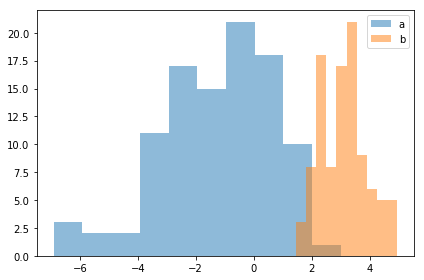
\includegraphics[width=\textwidth]{imgs/output_6.png}
        \caption{Histogram of a Feature-1 by Class Label }
        \label{fig:output_6}
    \end{subfigure}
    \begin{subfigure}[b]{0.6\textwidth}
        %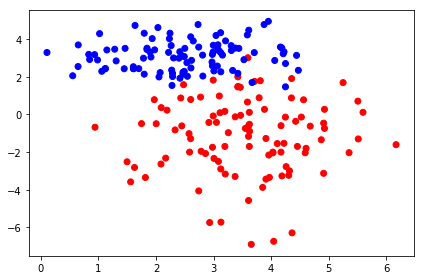
\includegraphics[width=\textwidth]{imgs/output_7.png}
        \caption{Datasets Scatter Plot by Color Class Label}
        \label{fig:output_7}
    \end{subfigure}
\end{figure}

\newpage

\subsection{Perceptron Model Training on Non-Linear Separable Data}

Knowing that the dataset in not linearly separable we can try to classify the data using the Perceptron algorithm following the same principles to train a model that apply to the linear separable dataset.  When training the perceptron model we need to a couple of parameters to ensure that the algorithm converges. Table.4 shows the number of iteration (Epochs) and the errors in each iteration, using a learning rate of $eta=0.45$ and for the iterations to train the model $n\_iter = 10$. 

\begin{table}[ht]
\centering
\caption{Perceptron Model - No. Iterations and Errors per Iterations}
\begin{tabular}{@{}lllllllllll@{}}
\toprule
\textbf{Epochs}     & 0 & 1 & 2 & 3 & 4 & 5 & 6 & 7 & 8 & 9 \\ \midrule
\textbf{No. Errors} & 1 & 4 & 4 & 2 & 3 & 2 & 2 & 4 & 3 & 2 \\ \bottomrule
\end{tabular}
\end{table}


\begin{figure}[ht]
\caption{Training the Perceptron Model}\label{fig:Perceptron01}
\centering
%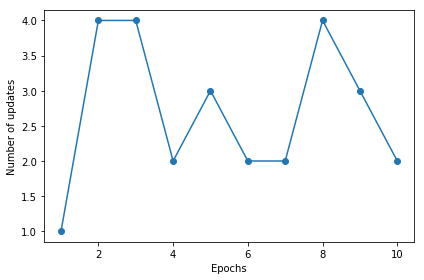
\includegraphics[width=13cm,height=12cm,keepaspectratio]{imgs/output_8.png}
\end{figure}

For this case it doesnt matter how much we change or tune the parameters in order to make the algorithm converge as the data is non-linearly separable. From the plot No. of Updates vs. Epochs below (Figure.6) we can visualize the how the Perceptron algorithm is not able to converges after 10 iterations (Epochs) we can try more iterations but still it wont converge as the data cant be divide in classes.


%----------------------------------------------------------------------------------------
%	SECTION 4 - MODEL SELECTION
%----------------------------------------------------------------------------------------

\section{AdelineSGD Model -- Titanic Dataset}

To predict passenger survival in the Titanic dataset scikit learn modules were used to create a train/test split of the data also to measure accuracy of the AdelineSGD algorithm the mean\_square\_ error model was used. Moreover the implementation of the code used in the report and code is from the book \textit{Python Machine Learning} by \textit{Sebastian Raschka}.

Prior to train the model there were some necessary data cleaning and transformation that are not going to be cover in this report. In general any null/missing values were filled with the mean or remove from the data also to classes were given a numeric value. Finally the clean dataset was normalize using the normalize module on scikit learn. 

\begin{figure}[ht]
\caption{Training the AdelineSGD Model}\label{fig:AdelineSGD}
\centering
%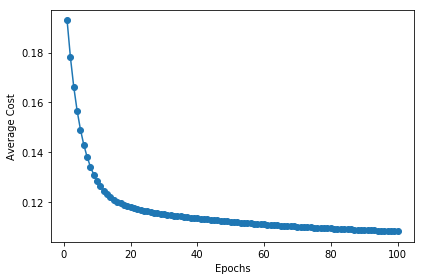
\includegraphics[width=\textwidth,keepaspectratio]{imgs/output_9.png}
\end{figure}

After performing all the mentioned transformation different AdelineSGD models were created variating the number of features, as many of the variable are categorical just the most relevant were used on the creating of the models. Figure.7 shows the average cost of AdelineSGD model with best performance (features: $age, fare$) after 100 iterations and learning rate of $0.0001$. In this case we can see how the model cost decrease with the number of iteration but it does not converge. To identify the features with best performance or set of features different combinations of AdelineSGD models and its performance were recorded in Table.5 we can see the different metrics for model performance which includes the number of features, average cost, mean square error calculated from the model prediction of the test data. 

From Table.5 we can determine that the last model (ada4) with 2 features  ($age, fare$) is the model that performs best when trying to predict passenger survival in the Titanic dataset for this particular train/test split. It its important to note that there may be other cases when other models have a better $MSE$ but in general the cost of each model is more or less around $~0.10$ to $0.12$.

\begin{table}[ht]
\centering
\caption{AdelineSGD Model Performance by No. Features}
\begin{tabular}{@{}cccc@{}}
\toprule
\multicolumn{1}{l}{\textbf{AdelineSGD Model}} & \multicolumn{1}{l}{\textbf{No. Features}} & \multicolumn{1}{l}{\textbf{Average Cost}} & \multicolumn{1}{l}{\textbf{MSE}} \\ \midrule
ada0 & 8 & 0.1072 & 0.6306 \\
ada1 & 4 & 0.1038 & 0.6157 \\
ada2 & 2 & 0.1201 & 0.6418 \\
ada3 & 2 & 0.1106 & 0.6007 \\
\textbf{ada4} & \textbf{2} & \textbf{0.1030} & \textbf{0.5448} \\ \bottomrule
\end{tabular}
\end{table}

%----------------------------------------------------------------
%	SECTION 5 - REFERENCE
%----------------------------------------------------------------

\section{Reference}

Cross-validation. 3.1. Cross-validation -- Scikit-Learn 0.19.0 Documentation, \url{http://scikit-learn.org/stable/modules/generated/sklearn.model_selection.train_test_split.html#sklearn.model_selection.train_test_split}

Model evaluation. 3.3.4.3. Mean squared error -- Scikit-Learn 0.19.0 Documentation, \url{http://scikit-learn.org/stable/modules/generated/sklearn.metrics.mean_squared_error.html}

Preprocessing Data. 4.3. Normalization -- Scikit-Learn 0.19.0 Documentation, \url{http://scikit-learn.org/stable/modules/preprocessing.html#normalization}

%----------------------------------------------------------------------------------------

\end{document}